\documentclass{cimento}
\usepackage{graphicx}

\def\al{\alpha}
\def\ga{\gamma}
\def\rh{\varrho}
\def\th{\vartheta}
\def\be{\beta}
\def\ph{\varphi}
\def\De{\Delta}
\def\Ph{\Phi}
\def\si{\sigma}
\def\un#1{\,{\rm #1}}
\def\subtitle#1#2{\vbox{\setbox0\hbox{#1}\copy0\hbox to\wd0{\hss#2\hss}}}
\def\abtitle#1#2{\vbox{\setbox0\hbox{#1}\hbox to\wd0{\hss#2\hss}\copy0}}
\def\d{{\rm d}}
\def\TODO#1{{\em #1}}


\begin{document}
%------------------------------------

\title{Soft Physics at the LHC with TOTEM}
\author{J.~Ka\v spar\from{ins:cern}\from{ins:fzu} on behalf of the TOTEM collaboration}
\instlist{%
	\inst{ins:cern} CERN, Geneva, Switzerland
	\inst{ins:fzu} Institute of Physics of the AS CR, Prague, Czech Republic
}
\PACSes{%
	\PACSit{13.85}{Hadron-induced high- and super-high-energy interactions (energy $> 10\ \rm GeV$)}
	\PACSit{29.40}{Radiation detectors}
}


\maketitle

\begin{abstract}
The physics programme and the detector apparatus of the TOTEM experiment is presented in the introduction. Then, the key running scenarios and their goals are summarized. The method to measure the total pp cross section is introduced. One of its essential parts, the extrapolation to $t=0$, is discussed in detail. In particular, an adequate parameterization and a treatment of Coulomb scattering is proposed. Eventually, extrapolation strategies for $\be^*=1535$ and $90\un{m}$ optics are presented. In the last section, TOTEM's plans for the LHC start-up are presented -- these include measurements of high $|t|$ elastic scattering and high-mass diffractive processes and studies of forward charged particle multiplicities.
\end{abstract}



\section{Introduction}\label{sec:intro}

The TOTEM experiment \cite{tdr,jinst,latino} is dedicated to forward hadronic phenomena. The tree pillars of its physics programme are: an accurate measurement of the total $\rm pp$ cross section, a measurement of elastic scattering in a wide kinematic range and studies of diffractive processes. 

The programme is touching one of the least explored and understood areas of hadronic physics. This fact can be well demonstrated by Fig.~\ref{fig:why}. The left plot shows several model predictions for elastic differential cross sections which differ by several orders of magnitude at large $|t|$ (four-momentum transfer squared). The right figure compiles data on the total pp cross section. Due to large uncertainties of cosmic ray experiments and conflicting Tevatron data \cite{tevatron1,tevatron2}, this data set can hardly favor any of the proposed theoretical descriptions over another. TOTEM shall shed some light onto those open questions by providing precise measurements -- see for instance the anticipated error bar for the total cross section in Fig.~\ref{fig:why}.

\begin{figure}[htb]
\centerline{\hss
	\includegraphics[height=0.4\textwidth]{../../EDS09/fig/elasticCrossSection_withAcceptance_bw}\hfil
	\includegraphics[height=0.4\textwidth]{../../EDS09/fig/sigma_tot}\hss
}%
\caption{Left: predictions of the elastic differential cross-section at a center-of-mass energy of $14\un{TeV}$ by several phenomenological models. Acceptance bands for the main optics (see Sec.~\ref{sec:scenarios}) are shown at the bottom. Right: a compilation of available data for the total pp cross section with a fit by the COMPETE collaboration \cite{cudell}. The anticipated ultimate precision ($1\%$) is shown in the bottom right corner.}%
\label{fig:why}%
\end{figure}

The challenging programme brings special requirements for the detector apparatus. In particular, {\em large pseudorapidity coverage} -- to detect most fragments from inelastic collisions and excellent {\em acceptance for surviving forward protons}. To accomplish this task, TOTEM comprises three subdetectors: the inelastic telescopes T1 and T2 and a system of Roman Pots (RP) for proton detection. This design results in a unique apparatus with an excellent pseudorapidity coverage, see Fig.~\ref{fig:acceptance} (a). The acceptance of the RPs can be further varied by using different optics, as will be discussed in the next section. The placement of telescopes T1 and T2 has been optimized to maximize the inelastic trigger efficiency (see Figs.~\ref{fig:acceptance}~(b) and (c)), which is of crucial importance for the total cross section measurement (discussed in Sec.~\ref{sec:tot meas}). For details on instrumentation see \cite{tdr, jinst}. 

\begin{figure}[htb]
\centerline{\hss
	\subtitle{\includegraphics[height=43mm]{../../EDS09/fig/acceptanceOverview_bw}}{(a)}\hskip4mm\hfil
	\subtitle{\includegraphics[height=42mm,width=43mm]{../fig/charged_multiplicity_minbias}}{(b)}\hskip4mm\hfil
	\subtitle{\includegraphics[height=42mm,width=43mm]{../fig/multiplicity_sd}}{(c)}\hss
}%
\caption{(a): The coverage of the three subsystems of TOTEM. The shown acceptance of the RPs refers to the $\be^*=1535\un{m}$ optics. For the other optics, the acceptance is shifted to lower pseudorapidity values, which narrows the gap between the RPs and T2.
(b) and (c): Pseudorapidity distributions of the charged particle multiplicity for non-diffractive (b) and single diffractive (c) inelastic collisions at the energy of $14\un{TeV}$. Let us remark that the main objective is to register most events -- and that is achieved with this design, even if some particles are missed.}%
\label{fig:acceptance}%
\end{figure}


%%%%%%%%%%%%%%%%%%
\section{Running scenarios}\label{sec:scenarios}

The forward protons, before being registered by the RP system, will pass through the lattice of the LHC magnets, and thus the observed hit pattern will depend on the accelerator settings (beam optics). In this way, the optics defines the acceptance and the resolution of the proton kinematics reconstruction (for details see chapter~6 in \cite{jinst}). Besides the optics, the beam collision parameters (such as luminosity) can be optimized for certain physics measurements. TOTEM plans to use the following three running scenarios.


\begin{enumerate}
\item {\em $\be^* = 1535\un{m}$} with ${\cal L} \approx (10^{28} \div 10^{29})\un{cm^{-2}s^{-1}}$. This is the ultimate optics for low $|t|$ elastic scattering and precise ($1\%$ error) total cross section measurement. The precision is made possible by very good angular resolution $\si(\th) \approx 0.3\un{\mu rad}$ (mainly due to the beam divergence). The momentum-loss ($\xi\equiv\De p/p$) resolution is $\si(\xi) \approx (2\div 10)\cdot10^{-3}$ for this optics.

\item {\em $\be^* = 90\un{m}$} with ${\cal L} \approx 10^{30}\un{cm^{-2}s^{-1}}$ is a universal optics allowing for measurement of elastic scattering (medium $|t|$ range), total cross section ($5\%$ uncertainty) and also for diffraction studies. The angular and momentum-loss resolutions are $\si(\th) \approx 1.7\un{\mu rad}$ and $\si(\xi) \approx (6\div 15)\cdot 10^{-3}$.

\item {\em $\be^* = (0.5 \div 3)\un{m}$} (standard optics for the general purpose experiments) are suited for high $|t|$ elastic scattering and various diffractive measurements. The relatively low cross sections of these processes require high luminosities ${\cal L} \approx (10^{32}\div10^{33})\un{cm^{-2}s^{-1}}$. The angular and momentum-loss resolutions are $\si(\th) \approx 15\un{\mu rad}$ and $\si(\xi) \approx (1\div 6)\cdot 10^{-3}$.
\end{enumerate}


See Fig.~\ref{fig:acceptances} for a comparison of proton acceptances for the above optics. Figure~\ref{fig:why} left shows that all the three scenarios are needed to measure elastic scattering in the wide $|t|$ range.

\begin{figure}[htb]
\centerline{\hss\hskip-1.5mm
	\abtitle{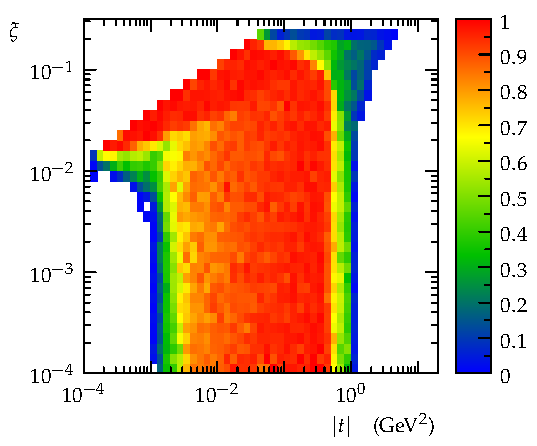
\includegraphics[height=44mm]{../fig/acceptance_1535}}{\qquad\quad$\be^* = 1535\un{m}$}\hfil
	\abtitle{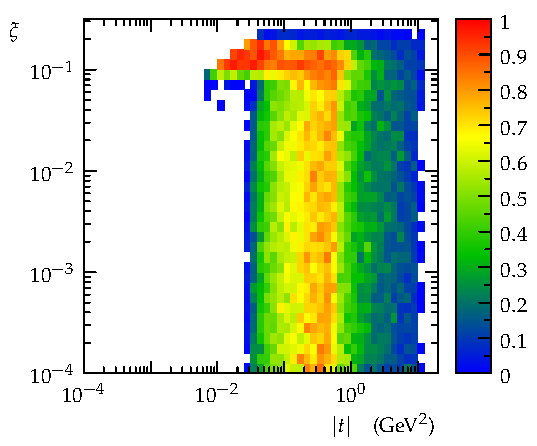
\includegraphics[height=44mm]{../fig/acceptance_90}}{$\qquad\quad\be^* = 90\un{m}$}\hfil
	\abtitle{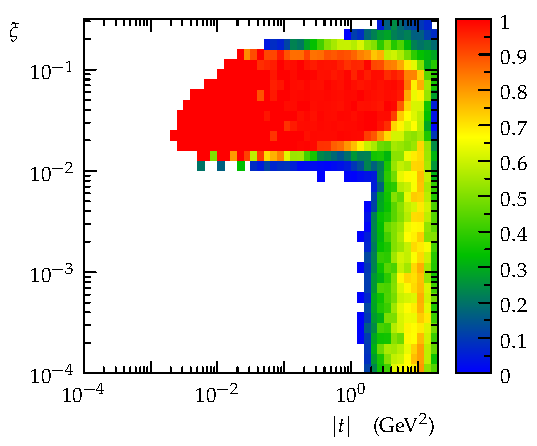
\includegraphics[height=44mm]{../fig/acceptance_2}}{$\qquad\quad\be^* = 2\un{m}$}\hss
}%
\caption{A comparison of RP acceptances for several optics at the center-of-mass energy of $14\un{TeV}$. Black color represents full acceptance while white zero acceptance. Note that the acceptance for elastic events can be read at the bottom horizontal axis ($\xi\to -\infty$).}%
\label{fig:acceptances}%
\end{figure}

All the scenarios mentioned have been conceived for the nominal LHC energy of $14\un{TeV}$. However, as it is planned in October 2009, the LHC will start up at a reduced energy of $7\un{TeV}$.% and optics $\be^*\approx2\un{m}$.
But still, one may assume that the main characteristics of the discussed scenarios will remain unchanged. The beginning of the LHC operation is scheduled for $\be^*\approx 2\un{m}$ runs. TOTEM plans for this period are presented in Sec.~\ref{sec:early}. Then, TOTEM intends to request the $90\un{m}$ optics as soon as possible. This optics is relatively easy to get (it does not require a special injection as the $\be^*=1535\un{m}$ one) and still allows for measurements throughout the entire physics programme -- note (e.g. in Fig.~\ref{fig:acceptances}) that all $\xi$'s are seen through a broad $|t|$ range. Moreover the $|t|$ range is shifted by nearly two orders down in comparison to the low $\be^*$ optics and therefore corresponding cross sections are much higher.



%%%%%%%%%%%%%%%%%%
\section{Measurement of the total cross section}
\label{sec:tot meas}

TOTEM intends to measure the total cross section by the {\em luminosity independent method}. It is based on the Optical Theorem:

\begin{equation}
\si_{\rm tot}(s) \propto \Im T^H(s, t = 0) \ ,
\end{equation}
%
relating the total cross section $\si_{\rm tot}$ to the hadronic\footnote{
There is obviously a second component due to the Coulomb scattering. Their interference is briefly discussed in Sec.~\ref{sec:extrapolation}.
} component of the elastic scattering amplitude $T^H(s, t)$. When it is complemented by common definitions for luminosity~$\cal L$ and rates~$N$
%
\begin{equation}\label{eq:def}
\rh = \left. \Re T^H\over\Im T^H \right|_{t=0}, \qquad {\d\si\over\d t} \propto |T^H|^2,\qquad \d N = {\cal L} \d\si,\qquad N_{\rm tot} = N_{\rm el} + N_{\rm inel},
\end{equation}
%
one can obtain relations for the total cross section and luminosity:
%
\begin{equation}\label{eq:lim}
\si_{\rm tot} = {1\over 1+\rh^2} {{\d N/ \d t|_{t=0}}\over N_{\rm el} + N_{\rm inel}}, \qquad\qquad {\cal L} = (1+\rh^2)\, {(N_{\rm el} + N_{\rm inel})^2\over {\d N/ \d t|_{t=0}}}\ .
\end{equation}
%
Here, $\d N/\d t|_{t=0}$ stands for elastic rate in the Optical Point (i.e. $t = 0$), which is to be obtained by an extrapolation procedure discussed in Sec.~\ref{sec:extrapolation}. $N_{\rm el}$ is the total elastic rate, which will be measured by the RPs and adjusted, again, by the extrapolation procedure. $N_{\rm inel}$ represents the total inelastic rate measured by the telescopes T1 and T2 (for more details see Sec.~2.2 in \cite{mario}).

The $\rh$ quantity can only be determined by an analysis of the Coulomb-hadronic interference (see below in Sec.~\ref{sec:extrapolation}) and there is only a small $|t|$ window, where these effects are significant enough. Moreover, for the energy of $14\un{TeV}$ this region is found around $t=1\cdot10^{-3}\un{GeV^2}$ which is on the very edge of TOTEM's acceptance. Therefore TOTEM might not be able to determine the $\rho$ value at the nominal LHC energy, unless allowed to insert the RPs closer than the standard $10$ beam-$\si$ distance (which would push the acceptance to lower $|t|$). 
For reduced energies, the prospects are much brighter as the interference region shifts towards higher $|t|$ values. Even if TOTEM was unable to resolve $\rho$, its value could be taken from external predictions (e.g. \cite{cudell}). Note that expected $\rho$ values are small $\approx 0.14$ and since $\rho$ enters the formulae Eq.~(\ref{eq:lim}) only via $1+\rh^2$, the influence of any uncertainty is small \cite{jinst,mario}.


%%%%%%%%%%%%%%%%%%%%%%%%%

\subsection{Extrapolation to $t = 0$}\label{sec:extrapolation}

\begin{figure}[htb]
\centerline{\hss
	\subtitle{\includegraphics[height=0.33\textwidth]{../../EDS09/fig/elasticCrossSection_low_bw}}{(a)}\hfil
	\subtitle{\includegraphics[height=0.33\textwidth]{../../EDS09/fig/elasticSlope_bw}}{(b)}\hss
	\subtitle{\includegraphics[height=0.33\textwidth]{../../EDS09/fig/phase_bw}}{(c)}\hss
}%
\caption{Model predictions for $E=14\un{TeV}$ in a low $|t|$ region. (a): predictions for the elastic differential cross section. (b): predictions for the elastic slope $B(s, t) = {\d\over\d t} \log {\d\si\over\d t}$. (c): predictions for the hadronic phase.}%
\label{fig:models low}%
\end{figure}


The value $\d\si/\d t|_0$ is, indeed, not accessible experimentally and thus an extrapolation from a higher $|t|$ region must be applied. A necessary condition for any successful extrapolation is a suitable parameterization. Looking at Fig.~\ref{fig:models low}, showing several model predictions in a low $|t|$ region, one can observe an {\em almost} exponential decrease of the elastic cross section up to $|t| \leq 0.25\un{GeV^2}$. This is further supported by the {\em almost} constant differential slope $B(s, t)$ in the quoted range\footnote{\label{fn:islam}
The model of Islam et al. is an exception which would be easily recognized (e.g. in large $|t|$ elastic scattering) and a different strategy would be applied.
}. The plot (c) hints that the phase of hadronic amplitudes can be described by a polynomial of a low degree. These arguments suggest that the following parameterization is adequate:
\begin{equation}
T^H(s, t) = e^{M(t)} e^{i P(t)},\ {\d\si\over\d t} = |T^{C+H}(s, t)|^2,\ \hbox{with }M, P\hbox{ polynomials for a fixed }s.\hskip-5mm
\label{eq:param}
\end{equation}
$T^{C+H}$ stands for the scattering amplitude of the combined Coulomb and hadronic forces and will be discussed below. The questions to be answered are: what is the optimal fit range and what is the optimal degree of the polynomials. It is obvious that if too many free parameters are introduced, they cannot be resolved with confidence. This is mainly a problem for the phase polynomial $P(t)$ since any phase information can only be resolved from a narrow Coulomb interference window, as discussed above. The optimal values shall give good results for most of the models considered; in this way the procedure can be regarded as model-independent.

So far, only the hadronic contribution $T^H$ to the elastic scattering has been discussed. It is clear that the Coulomb interaction will play a role and therefore must be taken into account. At the time being, there are two approaches to calculate scattering amplitudes $T^{C+H}$ for the combined interaction: the {\em traditional} (\`a la West-Yennie \cite{wy}) and the {\em eikonal} (see e.g. Kundr\' at-Lokaj\' i\v cek \cite{kl}). The traditional approach is based on rather constraining assumptions on the form of the hadronic amplitude, and furthermore it has recently been shown internally inconsistent \cite{wy inconsistent}.


%A comparison of the two approaches for several hadronic models can be found in Fig.~\ref{fig:coulomb}.

\iffalse
\begin{figure}[htb]
\centerline{\hss
	\includegraphics[height=0.4\textwidth]{../fig/coulombInterference_lin_bw}\hfil
	\includegraphics[height=0.4\textwidth]{../fig/R_bw}\hss
}%
\caption{Left: An illustration of Coulomb-hadron interference effects. Right: A comparison of West-Yennie and eikonal interference formulae (for $E=14\un{TeV}$). Acceptance starting points are also marked.}%
\label{fig:coulomb}%
\end{figure}
\fi

As mentioned in Sec.~\ref{sec:scenarios}, TOTEM plans to measure the total cross section with two optics: $\be^* = 1535\un{m}$ and $90\un{m}$. The lowest measurable $|t|$ values differ quite considerably (see Fig.~\ref{fig:acceptance} right and vertical marks in Fig.~\ref{fig:models low}) and therefore the extrapolation strategies differ as well.

For the $1535\un{m}$ optics, the Coulomb interference effects play a role and thus an interference formula must be applied (the eikonal one has been used in this study). The following configuration has been found optimal: quadratic $B(t)$ and constant phase with upper bound $|t| = 4\cdot10^{-2}\un{GeV^2}$. Preliminary results are shown in Fig.~\ref{fig:extrapol}~(a). One can see that most models lie within a band $\pm 0.2\%$ (except for the model of Islam et al. -- see footnote \ref{fn:islam}).

As for what concerns the $90\un{m}$ optics, the Coulomb effects are negligible and therefore the phase parameterization becomes irrelevant\footnote{%
The $T^{C+H}$ coincides with $T^H$ and the phase factor $\exp{(i P(t))}$ cancels out when differential cross section is calculated according to the Eq.~(\ref{eq:param}).
}. On the other hand, the horizontal $t$ component $t_x$  can be resolved with a limited resolution only -- see Fig.~\ref{fig:extrapol}~(b). Since $t = t_x + t_y$, the considerable uncertainties propagate to the full $t$ distribution. A number of solutions might be suggested.

\begin{enumerate}
\item Use the $t$-distribution (i.e. $\d\si/\d t$) despite large uncertainties.

\item Using azimuthal symmetry, one can ``transform'' a $t_y$-distribution in a $t$-distribution:
%$$t = t_x + t_y,\qquad t_x = t\cos^2\ph,\quad t_y=t\sin^2\ph$$
$${\d\si\over\d t_y} = {\d\si\over\d t_x} \quad \Rightarrow \quad {\d\si\over\d t}(t) \propto \int\limits_t^0 \d u\, {\d\si\over\d t_y}(u)\, {\d\si\over\d t_y}(t - u)\ .$$
However, since low $|t_y|$ information is missing (out of acceptance), an extrapolation step would be needed just for this transformation.

\item ``Transform'' a $t$-parameterization in a $t_y$-parameterization and fit it directly through $t_y$ data:
$$t_y = t\,\sin^2\ph, \hbox{ with }\ph\hbox{ uniformly distributed} \quad \Rightarrow \quad {\d\si\over\d t_y}(t_y) = {2\over\pi} \int\limits_{0}^{\pi/2} {\d\ph\over\sin^2\ph}\ \ {\d\si\over\d t}\!\left(t_y\over\sin^2\ph\right)$$
Considering a parameterization of type Eq.~(\ref{eq:param}), one can derive an approximate formula:
$${\d\si\over\d t} = e^{a\, +\, bt\, +\, ct^2\, +\, \ldots} \quad\Rightarrow\quad {\d\si\over\d t_y}(t_y) \approx {1\over\sqrt{\pi}}\, {e^{a\, +\, bt_y\, +\, ct_y^2\, +\, \ldots}\over\sqrt{|b\,t_y|}}$$
which can be justified provided the non-linear terms in the exponent ($ct^2,\, \ldots$) do not give an essential contribution -- which is the case, see Fig.~\ref{fig:models low}.
\end{enumerate}

	
Eventually, the third approach has been chosen and a cubic polynomial with an upper bound of $|t| = 0.25\un{GeV^2}$ has been found optimal. Preliminary results are plotted in Fig.~\ref{fig:extrapol}~(c). Most models fall in a band between $-1\%$ and $-3\%$ (Islam's model being again an exception -- see footnote \ref{fn:islam}). The overall offset of $-2\%$ is a consequence of the beam divergence and can be corrected in the data analysis.

\begin{figure}[htb]
\centerline{\hss
	\subtitle{\includegraphics[height=0.33\textwidth]{../../EDS09/fig/extrapolation1535}}{(a)}\hfil
	\subtitle{\includegraphics[height=0.33\textwidth]{../../EDS09/fig/tError90}}{(b)}\hfil
	\subtitle{\includegraphics[height=0.34\textwidth]{../../EDS09/fig/extrapolation90}}{(c)}\hss
}%
\caption{(a): the extrapolation deviation as a function of fit's lower bound for the $\be^* = 1535\un{m}$ optics.
(b): comparison of $t_x$ and $t_y$ resolutions for the $\be^* = 90\un{m}$ optics.
(c): the extrapolation deviation for the $90\un{m}$ optics.
All plots are based on {\em preliminary} simulation/reconstruction data.}%
\label{fig:extrapol}%
\end{figure}




%%%%%%%%%%%%%%%%%%%%%%%%%

\subsection{Inelastic rate}\label{sec:early}

The inelastic rate $N_{\rm inel}$ (in Eq.~(\ref{eq:lim})) is to be measured by the forward trackers T1 and T2. In order to maximize the detection efficiency a number of trigger strategies is foreseen, see e.g. Sec.~2.2 in \cite{mario}. The dominant contribution of trigger losses is expected to arise from low-mass single or double diffractive events. To correct for this deficiency, an extrapolation procedure has been established (details can be found in Sec.~6.2.2 in \cite{jinst}).

%Extrapolation to lower masses. The argument to identify any exceeding resonances.


%%%%%%%%%%%%%%%%%%%%%%%%%

\begin{figure}[htb]
\hbox to\hsize{\hss
	\subtitle{\raise7mm\hbox{\includegraphics[width=4cm]{../fig/sd_high_mass_var}}}{(a)}\hfil
	\subtitle{\raise7mm\hbox{\includegraphics[width=4cm]{../fig/dpe_high_mass_var}}}{(b)}\hfil
	\subtitle{\includegraphics[width=50mm]{../fig/high_mass_SD}}{(c)}\hss
}%
\caption{(a) and (b): characteristic event structures of high-mass single diffraction (a) and double pomeron exchange (b). The boxes in the upper part present pseudorapidity vs.\ azimuthal angle charts. The diagrams in the bottom show momenta of particles in sample events, together with rapidity gaps $\De\eta$ between surviving protons $\rm p$ and edges of the diffractive system $\rm X$.\hfil\break
(c): pseudorapidity distribution of charged particles produced in single diffractive events with $\xi$ range compatible with the RP acceptance in the LHC start-up scenario. In this simulation, only intact protons with negative pseudorapidity have been considered. The shaded vertical bands represent the coverage of the telescopes T1 (blue) and T2 (red).
}%
\label{fig:high mass diff}%
\end{figure}

\section{Early measurements}\label{sec:early}

As of October 2009, the LHC schedule counts on first physics collisions at the center-of-mass energy of $\sqrt{s} = 7\un{TeV}$ and $\be^*\sim2\un{m}$. The expected RP acceptance and resolution for this scenario are similar to the nominal energy case, see Sec.~\ref{sec:scenarios}. That means $\xi$ acceptance $0.02 < \xi < 0.18$ and resolution $\si(\xi) < 6\cdot10^{-3}$, elastic acceptance $2 < |t| < 20\un{GeV^2}$ and resolution $\si(t)\approx 0.2/\sqrt{|t|}$. These parameters are suitable for the physics studies listed below.
\begin{itemize}
\item The vertical RPs will measure {\em high $|t|$ elastic scattering}.

\item Given the range where $\xi$ can be determined by (horizontal) RPs, TOTEM will measure spectra of {\em high-mass diffractive processes}. For single diffraction,the mass spectrum $\d\si^{\rm SD}/\d M$ could be measured for masses $1\un{TeV} < M < 3\un{TeV}$. 
%$, $\si(M) / M \approx 1.5\div 15\%$
For double pomeron exchange\footnote{Here, the term ``double pomeron exchange'' is used as a synonym to central diffraction.}
the distribution $\d\si^{\rm DPE}/\d M$ will be available for masses $0.14\un{TeV} < M < 1.3\un{TeV}$.
%, $\si(M) / M \approx 3\div 30\%$
See Fig.~\ref{fig:high mass diff}~(a) and (b) for typical event topologies for these processes.

The value of $\xi$ can be alternatively determined by the telescopes T1 and T2. When an edge of a rapidity gap is detected in the telescopes (see the band around $\eta\approx -5$ in Fig.~\ref{fig:high mass diff}~(c)), the gap size $\De\eta$ can be related to the momentum loss by $\De\eta\approx - \log\xi$. In this way, the accessible mass regions can be extended to lower values.

\item  The telescopes T1 and T2 alone can be used for studies of {\em forward charged particle multiplicities}.
%TODO: important for MC tuning and !!??
%See Fig.~\ref{fig:multiplicity}
\end{itemize}




\iffalse
\begin{figure}[htb]
\hbox to\hsize{\hss
	\includegraphics[width=50mm,height=45mm]{../fig/mc_charged_multiplicity}\hss
}%
\caption{Large uncertainties in Monte Carlo predictions of forward charged multiplicity.}%
\label{fig:multiplicity}%
\end{figure}
\fi




\begin{footnotesize}
\begin{thebibliography}{99}

\bibitem{tdr}
	TOTEM: Technical Design Report, CERN-LHCC-2004-002 (2004); addendum CERN-LHCC-2004-020.

\bibitem{jinst}
  G.~Anelli {\it et al.}  [TOTEM Collaboration],
  %``The Totem Experiment At The Cern Large Hadron Collider,''
  JINST {\bf 3}, S08007 (2008).

\bibitem{latino}
  G.~Latino  [TOTEM Collaboration],
  ``The TOTEM Experiment at LHC,''
  %By TOTEM Collaboration (Giuseppe Latino for the collaboration). May 2008. 16pp.
  22nd Les Rencontres de Physique de la Vallee d'Aoste, Aosta Valley, Italy (2008).
  %Published in *La Thuile 2008, Results and perspectives in particle physics* 631-646

\bibitem{tevatron1}
  F.~Abe {\it et al.}  [CDF Collaboration],
  %``Measurement of the $\bar{p}p$ total cross-section at $\sqrt{s} = 546$ GeV
  %and 1800-GeV,''
  Phys.\ Rev.\  {\bf D50} (1994) 5550.

\bibitem{tevatron2}
  N.~A.~Amos {\it et al.}  [E710 Collaboration],
  %``Measurement of $\rho$, the ratio of the real to imaginary part of the
  %$\bar{p} p$ forward elastic scattering amplitude, at $\sqrt{s}$ = 1.8-TeV,''
  Phys.\ Rev.\ Lett.\  {\bf 68} (1992) 2433.

\bibitem{cudell}
  J.~R.~Cudell {\it et al.}  [COMPETE Collaboration],
  %``Benchmarks for the forward observables at RHIC, the Tevatron-run II and
  %the LHC,''
  Phys.\ Rev.\ Lett.\  {\bf 89} (2002) 201801.
  %[arXiv:hep-ph/0206172].

\bibitem{mario}
	M.~Deile  [TOTEM Collaboration],
	{\it Total cross-section measurement and diffractive physics with TOTEM},
	12$^{\rm th}$ International Conference on Elastic and Diffractive Scattering,
	%Blois07, Forward physics and QCD* 153-159
	Hamburg (2007)

\bibitem{wy}
  G.~B.~West and D.~R.~Yennie,
  %``Coulomb interference in high-energy scattering,''
  Phys.\ Rev.\  {\bf 172} (1968) 1413.

\bibitem{kl}
  V.~Kundr\' at and M.~Lokaj\' i\v cek,
  %``High-energy scattering amplitude of unpolarized and charged hadrons,''
  Z.\ Phys.\ {\bf C63} (1994) 619.
  %%CITATION = ZEPYA,C63,619;%%

\bibitem{wy inconsistent}
  V.~Kundr\' at, M.~Lokaj\' i\v cek and I.~Vrko\v c,
  %``Limited validity of West and Yennie integral formula for elastic scattering
  %of hadrons,''
  Phys.\ Lett.\ {\bf B656} (2007) 182.
  %[arXiv:0706.0827 [hep-ph]].
  %%CITATION = PHLTA,B656,182;%%

\iffalse
\bibitem{simone}
	S.~Giani [TOTEM Collaboration],
	{\it Diffraction at TOTEM},
	13$^{\rm th}$ International Conference on Elastic and Diffractive Scattering,
	CERN (2009).

\bibitem{gennaro}
	G.~Ruggiero [TOTEM Collaboration],
	{\it TOTEM},
	13$^{\rm th}$ International Conference on Elastic and Diffractive Scattering,
	CERN (2009).

\bibitem{alfa}
	ATLAS-ALFA: Technical Design Report, CERN-LHCC-2008-004 (2008).

\bibitem{millepede}
	V.~Blobel, Millepede II documentation at http://www.desy.de/$\sim$blobel/Mptwo.pdf\ .

\bibitem{ua5}
  G.~J.~Alner {\it et al.}  [UA5 Collaboration],
  %``Antiproton-proton cross sections at 200 and 900 {GeV} c.m. energy,''
  Z.\ Phys.\  {\bf C32} (1986) 153.
  %%CITATION = ZEPYA,C32,153;%%

\bibitem{isr}
  U.~Amaldi {\it et al.},
  %``The Energy dependence of the proton proton total cross-section for
  %center-of-mass energies between 23 and 53 GeV,''
  Phys.\ Lett.\  {\bf B44} (1973) 112.
\fi

\end{thebibliography}

\end{footnotesize}


\end{document}
